\versoquote{ἀγεωμέτρητος μηδεὶς εἰσίτω.}{Ἀκαδημία}
\chapter{Introduction}
\loftchap{Introduction}
\chapterprecis{He writes some words. What happens next will flaw you.}

\thought{The ability to create a} device whose macroscopic quantities are quantum variables is advantageous for a myriad of reasons, one in particular is the development of a quantum computer.
Constructing circuits which invoke the tunnelling effect of Josephson junctions (JJs) in conjunction with superconducting phenomena manifest controllable quantum properties which can be exploited to this end.\nomdef{AJJ}{JJ}{Josephson junction}
However, the use of quantum bits (qubits) for computation is dependent on the ability to operate them in an essentially isolated environment, \ie the system must operate over coherent states.
The phenomenon of decoherence refers to the instability of a quantum state of a system when it interacts with the surrounding environment.
In general, the stronger the interaction with the environment, the quicker the quantum state decoheres.
Removal or control of these defects is required before quantum computers using superconducting circuit architecture can be realised.

\section{A Qubit Primer}
A quantum bit differs from its classical counterpart (the bit) in a number of ways.
A bit can be represented by either 0 or 1, where the state of the system exists in only one of these positions at any given time, and are usually manifestations of a potential difference inside some macroscopic circuit.
Qubits on the other hand are a two-level quantum mechanical system, existing in a Hilbert space or projective Hilbert space.
In a given orthonormal basis, the state vectors $\ket{0}$ and $\ket{1}$ represent the two level nature of the system (perhaps corresponding to the spin-up and spin-down states of an electron for example).
In addition to the state vectors, a qubit may exist in a superposition of the $\ket{0}$ and $\ket{1}$ basis, which is known as a pure state.

The Bloch sphere \cite{Bloch1946} is a useful tool to represent qubit states, with the poles interpreted as the two basis vectors, and the points on the surface of the sphere corresponding to the pure states of the system.
\Cref{fig:bloch} illustrates this for an arbitrary pure state $\ket{\psi}$.
\begin{figure}[htp]
\resizebox{0.5\textwidth}{!}{\includestandalone{figures/bloch}}
\caption[Bloch Sphere]{\label{fig:bloch}The Bloch Sphere: a geometrical representation of the pure state space of a two-level quantum system in an arbitrary Hilbert space $\hat{e}_{\{1,2,3\}}$. This example shows a pure state $\ket{\psi}$ calculated using \cref{eq:purestate} with $\cramped{\phi=\frac{\pi}{3}}$ and $\cramped{\theta=\frac{2\pi}{9}}$. }
\end{figure}

The physical state of the system is not affected by global phase factors, thus in the complex superposition of the basis vectors, the coefficient of $\ket{0}$ is real and non-negative.
This means the pure state can be represented as
\begin{equation}
\ket{\psi} = \cos\left(\theta\right) \ket{0} \, + \, e^{i \phi}  \sin\left(\theta\right) \ket{1},
\label{eq:purestate}
\end{equation}

where $\cramped{-\frac{\pi}{2} \leq \theta < \frac{\pi}{2}}$ and $0 \leq \phi < 2 \pi$.

The interior region of the Bloch sphere represents qubit mixed states: statistical ensembles of pure states.
As these states cannot be described by ket vectors, a density matrix must be defined
\begin{equation}
\rho = \sum_k p_k \ket{\psi_k} \bra{\psi_k},
\end{equation}

where $p_k$ is the fraction of each pure state $\psi_k$ represented in the mixture.

As a qubit state evolves through time, the equation of motion can be written as
\begin{equation}
i\hbar \frac{\mathrm{d}\rho}{\mathrm{d}t} = \com{H}{\rho}
\label{eq:tevqubit}
\end{equation}
which evolves entirely due to the dynamics of a Hamiltonian $H$,
provided the qubit is completely isolated from any environmental perturbations.

\subsection{Interaction With the Environment}\label{sec:envint}

Environmental noise sources are seldom completely removed from qubit operations and in practically all current designs, interaction with this uncontrolled, perturbative source is unavoidable.
Noise being an umbrella term for thermal radiation, collisions, lattice vibrations or any other form of energy dissipation phenomena which causes the time evolution of the qubit to become irreversible: taking away information about the state being represented.
This (primarily) decreases the quantum coherence of the system and measurements in turn deteriorate.

Qubit dynamics can therefore no longer be considered as a unitary evolution described by the von Neumann equation \cref{eq:tevqubit}, but instead as an open quantum system.
A master equation approach is therefore required to further describe qubit time evolution as it interacts with the environment.
For simplicity, we assume that environment perturbations to our qubit come from an arbitrarily large bath of uncorrelated noise sources with a uniform frequency spectrum.
Also, interactions between the system and environment are brief with respect to ordinary system dynamics determined by the hamiltonian $H$.
These conditions describe the most general type of Markovian and time homogeneous master equation, the Lindblad form~\cite{Lindblad1976}
\begin{equation}
\frac{\mathrm{d}\rho}{\mathrm{d}t} =-\frac{i}{\hbar}\com{H}{\rho}+\sum_{k} \Gamma_k\left(L_k\rho L_k^\dagger-\frac{1}{2}\left\{L_k^\dagger L_k, \rho\right\}\right)
\end{equation}
where the Lindblad operators $L_k$ and the rates $\Gamma_k$ determine
how the environment interacts with the system.

It can be shown that a qubit damped via environment interaction looses coherence on two time scales ~\cite{Stenholm2005}:
\begin{equation}
\frac{1}{T_1} = \Gamma_+ + \Gamma_-, \qquad \frac{1}{T_2} = \gamma + \frac{\Gamma_+ + \Gamma_-}{2}, \qquad \frac{\Gamma_+}{\Gamma_-} = \exp\left(-\frac{\hbar \omega}{k_B T}\right).
\end{equation}
The times $T_1$ and $T_2$ are called the \textit{energy (longitudinal)} and \textit{phase (transverse)} relaxation times respectively.
$T_2$ has an additional contribution $\gamma$ which is a contribution due to random movement of the relative phase caused by perturbations of the environment.

These relaxation processes are the ultimate optical to the realisation of a working qubit architecture.
Level populations tend to be more robust than the phase (which is easily disturbed by the environment), so generally $T_2 < T_1$.
This time equates to a fundamental limit in most experimental systems and is often called the \textit{decoherence} time.

\section{Qubit Architectures}
Physical qubit implementations can nominally be broken up into four categories: ultracold atoms, spin-based systems, quantum optics and superconducting circuits; each with their own strengths and weaknesses.

The following is not an exhaustive list or discussion of qubit conceptions, it is presented to the reader as an overview of the efforts in the wider quantum information science community before focusing on specific devices relevant to this thesis.

A comprehensive roadmap containing many of the advances in quantum computing (unfortunately only up to 2004) can be found via \onlinecite{qist2004}.

\subsection{Ion Traps}
Electromagnetic fields, light waves or a combination of both can be used to suspend and isolate charged atomic particles (ions) in free space~\cite{Paul1990}.
Ion trapped qubits~\cite{Cirac1995} exploit stable electronic or spin states of the ion to store information, which in turn can be processed and transmitted through the collective quantised motion (via the Coulomb force) of other ions in the trap.

Single qubit operations can be invoked by spin-phonon coupling (for example) induced by a laser pulse.
Multiple entangled qubits can be coupled through internal states and external motion states in a similar fashion.

Ion traps show significant promise for the future of quantum information processing, as architectures with many coupled qubits are already experimentally accessible.
Fundamental gating operations such as the C-NOT have also been demonstrated with high fidelity.

\subsection{Nitrogen-Vacancy Center of Diamond}

The nitrogen vacancy (NV$^-$) center~\cite{Gruber1997} is seemingly the most studied crystalline defect in existence.
Application areas include ultrasensitive sensing of electric, magnetic and strain fields; biological imaging and sensing; and a room temperature, solid state qubit architecture.

The center exhibits atom-like properties: long-lived spin quantum states and well-defined optical transitions, whilst encased in a robust solid-state device.
Both its bound electrons and nearby nuclear spins can be addressed using optical transitions much like the atomic states in ion traps.
On-chip wiring and waveguides govern fast electrical and magnetic control which exploits the solid state nature of the diamond lattice.

These unique properties give rise to an electron spin lifetime longer than that of a trapped ion (at low temperatures)~\cite{Jarmola2012} and coherence times larger than a second at room temperature if nearby nuclear spins are utilised~\cite{Maurer2012}.

\subsection{Quantum Dots}
Quantum dots are made of semiconductor material and are used to contain and manipulate electrons in microcavity modes, which in turn behave as an \textit{artificial} atom.
Manipulation can come about via electronic~\cite{Chang1974} or optical~\cite{Dingle1974} methods, and the resultant coherent system states can be used as a qubit.

Quantum dots are relatively simple to construct and control with modern semiconductor technology, and their environmental coupling is rather weak providing long coherence times.
Even early schemes hinted at the possibility of coupling more than 100 qubits using a single cavity mode and laser fields to mediate coherent interactions between distant quantum dot spins~\cite{Imamoglu1999}, although this has proved difficult in practice.

\subsection{Superconducting Circuits}

Microscopic degrees of freedom (\eg spin) of ions, crystal defects or artificial atoms are well isolated from the environment and therefore operate as good qubits.
However, inter-qubit coupling in these systems becomes complex at scale and fast gating operations required for computation is a task that for many architectures introduces decoherence.
Hence while the qubit itself is isolated, the quantum computer suffers as a whole.

The superconducting circuit architecture is different from these systems, as it instead uses a collective electrodynamic mode of macroscopic electrical elements.
Therefore, gating is no longer an issue: simple electrical elements (capacitors, inductors \etc) can be coupled to the qubits directly.
Adaptation of nano-fabrication techniques developed in the semiconductor industry to build scalable integrated quantum devices once operational designs are developed is therefore possible.
A tradeoff exists though, as the qubits are no longer easily isolated from the surrounding environment.

The basic features of a superconducting qubit circuit are ultra-low dissipation (from superconductivity), ultra-low noise (from low temperature) and non-linear, non-dissipative elements (specifically in the form of the Josephson junction).

Superconductivity allows electron flow with almost no resistance.
Type I superconductors are primarily used in circuit construction due to their simplicity compared to their Type II counterparts (aluminium is a popular choice), which only operate in the superconducting regime at low temperature.
Cooling the system to this level is advantageous from a noise argument as well: qubits must be cooled to temperatures where the typical energy $k_B T$ of thermal fluctuations is much less that the energy quantum $\hbar \omega_{01}$ associated with the transition between the $\ket{0}$ and $\ket{1}$ states.
This frequency is nominally in the $5\!-\!20$ GHz range, thus the operating temperature $T$ must be around $20$ mK or lower.

There are three basic types of superconducting qubits which form around the Josephson junction.
Each design is an attempt to minimise the detrimental effect of a `residual offset charge', that manifests as a consequence of a pre-existing charge on the capacitor at the time it is wired to the inductor (see \cref{fig:qubit} below) in order to fabricate the qubit.

The simplest idea to mitigate this issue is the Cooper pair box~\cite{Nakamura1999,Bouchiat1998}, which biases the JJ with a voltage in series with a gate capacitor.
Circuits derived from this method are commonly called charge qubits~\cite{Makhlin2001,Vion2002} although it's important to note that the name does not imply information is encoded in the charge of the system, but instead refers to the controlling variable of the system.
The transmon~\cite{Wallraff2004, Schreier2008} is a relatively new qubit design that stems from the original charge qubit ideas, but shrinks the cooper pair box size in an attempt to squelch decoherence sources.

The second circuit type (the RF-SQUID~\cite{Barone1982}) can be considered the dual of the Cooper pair box, employing a superconducting transformer in place of the aforementioned gate capacitor.
Designs utilizing this method are referred to as Flux qubits~\cite{Mooij1999,VanderWal2000,Chiorescu2003}, again this is because a controllable external flux field is imposed on a superconducting loop across the JJ rather than the idea that information is stored in the magnetic moment of the qubit.

Another method to minimise the effect of offset charge is to bias the JJ with a fixed DC current source.
Implementation of this design is referred to as the Phase qubit~\cite{Clarke1988,Martinis2002}, a circuit diagram of which is depicted in \cref{fig:qubit}.

\begin{figure}[htp]
\resizebox{0.75\textwidth}{!}{\includestandalone{figures/qubit}}
\caption[Phase Qubit Circuit Diagram]{\label{fig:qubit}Circuit diagram of a phase qubit and readout components. This schematic is representational of current designs, based on improvements made in \onlinecite{Simmonds2004}.}
\end{figure}

This design has a highly capable readout mechanism and multi-qubit scaling arrangements are promising.
Thus the possibility of a functioning quantum computer using it is encouraging with only one major caveat: the system is mired with decoherence causing defects.
In fact, much of the superconducting qubit community has transitioned from active phase qubit experimentation to the transmon because of this phenomena.

On the other hand, this design is very useful for studying these decoherence sources (\textit{vide infra} \cref{sec:probes}) and therefore the most relevant architecture to study throughout this thesis.

\section{Josephson Junctions}
A normal LC circuit generates a parabolic potential, which in energy terms is a harmonic oscillator: transitions between neighboring excited states are degenerate.
If we wish to use this kind of circuit as a qubit, the transition between state $\ket{0}$ and $\ket{1}$ must be sufficiently different to the higher-lying eigenstates of the system.

\Cref{fig:qubit} depicts an LC circuit in parallel with a barrier component  \resizebox{!}{0.6em}{\includestandalone{figures/jjcomponent}}.
\nomdef{ALC}{LC}{Inductor-Capacitor circuit, generates a harmonic oscillator}
This symbol represents the Josephson junction, which at low temperature is a strongly non-linear, non-dissipative circuit element\footnote{One reason why the JJ is so ubiquitous in superconducing devices is that for many years it was the \textit{only} non-linear component. Recently the quantum phase slip junction~\cite{Bezryadin2000,Mooij2006,Astafiev2012} (effectively the dual of the JJ) has been showing great promise as well.}.
In fact, a JJ behaves as a pure non-linear inductor in parallel with a capacitor resulting from the parallel plate capacitance inherent in the junctions' construction (see \cref{fig:jjdiagram} below).
These features give rise to an anharmonic oscillator, a readable energy spectrum and the possibility of a working qubit.

This is all possible because of the Josephson effect~\cite{Josephson1962,Josephson1965}, which is one of the most significant examples of macroscopic quantum phenomena presently known.
Current flow between two superconductors separated by a thin insulating layer (\ie a JJ) is possible even in the absence of electrical voltage drop across the junction, making this phenomena a \textit{supercurrent}.
Cooper pairs tunneling through the insulating barrier are the cause of this supercurrent, which manifests macroscopically, but depends on the quantum phase of the system.

Josephson junctions may be constructed from any superconducting material with any insulating or non-superconducting metal barrier to invoke a weak link coupling.
A popular material choice involves the use of aluminium as the superconducting material, and an amorphous oxide layer as an insulating barrier -- an illustration of which is depicted in \cref{fig:jjdiagram}.

\begin{figure}[htp]
\resizebox{0.75\textwidth}{!}{\includestandalone{figures/jjdiagram}}
\caption[Josephson Junction Schematic]{\label{fig:jjdiagram}Schematic of a Josephson junction constructed with two superconducting thin films of aluminium and an amorphous \ce{AlO_x} tunnel barrier.}
\end{figure}

For further discussion of the theory behind, and the engineering prospects of the Josephson junction, see the the great review article by \citeauthor{Makhlin2001}~\cite{Makhlin2001}.

\subsection{Formation Process}\label{sec:formation}

Shadow evaporation is a common technique used to fabricate systems such as this, where two metallic layers are deposited from different angles with an intervening oxidation step.
This is usually performed using a Dolan bridge, which obscures part of the substrate during each metal deposition step \cite{Dolan1977}.
It has more recently been shown that junction fabrication can be performed without the requirement of this bridge \cite{Lecocq2011}.
Regardless of the process chosen, the oxidation of the aluminium does not result in a set of crystalline monolayers, but a non-uniform amorphous layer varying in stoichiometry~\cite{Park2002, Tan2005}, density~\cite{Barbour1998} and thickness~\cite{Gloos2003,Aref2014,Zeng2014} (nominally $\sim\!2$ nm).  Although epitaxial growth of aluminium-oxide barriers has been demonstrated~\cite{Oh2006}, this technique is not yet mainstream as it is considerably more difficult than conventional shadow mask evaporation.


\section{Investigating Decoherence Sources}

Essentially a $1/f$ \cite{Dutta1981} discussion, tying back to \cref{sec:envint}.


\subsection{NOTES ON DECOHERENCE}
Standard open quantum systems theory:  $1/f$ noise because TLS are considered to be an ensemble, causing background fluctuations. (adds additional dephasing mechanism $\gamma$ in $T_2$)


Strongly coupled TLSs. Cannot be considered as a simple Lindbladian decoherence channel,
because TLS is coherent and coupled more strongly to the qubit than other processes.
Time scales associated with TLS-Qbit coupling ($S_{max}$) is shorter than all other decoherence time scales.

Therefore we have to consider the TLS as its own quantum system `in isolation'.
This thesis asks questions about the properties of the TLS derived from the material properties of the JJ it resides in.



\section{Strongly Coupled Two Level Systems}
Look at \cite{Enss2005} in depth here.


One of the key decoherence channels facing superconducting qubits and other Josephson junction devices are certain bistable material defects (herein defined as two-level systems or TLSs)~\cite{Dutta1981, Shnirman2005}.
Experiments have probed these defects directly and shown them to be stable, controllable and have relatively long decoherence times~\cite{Simmonds2004, Neeley2008, Shalibo2010, Lupascu2009, Lisenfeld2010, Gunnarsson2013}.
A variety of phenomenological models exist~\cite{Martinis2005, DeSousa2009, Sendelbach2008, Faoro2007,Ku2005} which can describe the properties of these defects, although their true microscopic origin remains elusive.
In particular, the superconducting phase qubit is mired by decoherence via multiple TLS sources and as such cannot operate long enough for surface code to correct errors caused by this process.


Bistable defects in glasses and amorphous solids in general have been understood for some time~\cite{Anderson1972}.
Amorphous insulating barriers (either in the form of Josephson junctions or simply a native oxide) form an integral part of superconducting circuits, so it comes as no surprise that TLSs are often considered to be an important source of noise in these circuits~\cite{Dutta1981, Shnirman2005, Martinis2005}.


A common and important source of decoherence is the environmental two-level system (TLS)~\cite{Dutta1981, Shnirman2005}.
\nomdef{ATLS}{TLS}{Two level system}
Experiments have probed these defects directly and shown them to be stable, controllable and have relatively long decoherence times,~\cite{Simmonds2004, Neeley2008, Shalibo2010, Lupascu2009, Lisenfeld2010, Gunnarsson2013} although little is known about their true microscopic nature.


\subsection{Qubits as Probes of TLSs}\label{sec:probes}


Developments in controllable qubit architecture (charge, flux and phase) has enabled the study of so-called `strongly coupled defects'~\cite{Neeley2008, Lupascu2009, Lisenfeld2010}.
These defects have comparable resonance frequencies to the qubit circuit and coupling strengths as well as decoherence times long enough to allow coherent oscillations between the qubit and TLS.
Probing individual defects has promoted their bistable nature from hypothesis to observable fact, as well as providing clues to their microscopic origin.


\begin{figure}[htp]
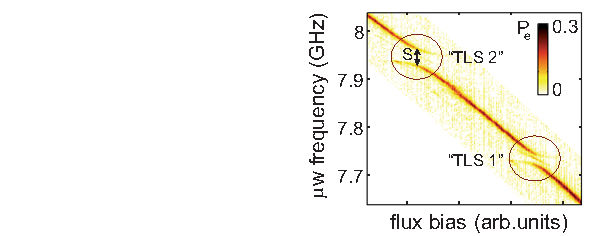
\includegraphics[width=0.6\textwidth]{figures/alclisenfeld2010}
\caption[ALC]{\label{fig:alc}ALC from \citeauthor{Lisenfeld2010}.}
\end{figure}

As stated in \cref{sec:formation}, the amorphous oxide is the general case for construction.
As such we need to investigate this, esp bc \cite{Oh2006}.
as a formation which needs to be investigated predominantly, in order to obtain results from simulation which are applicable to future fabrication work.

\subsection{Phenomenological Models}

Many phenomenological theories attempting to describe them exist; including charge dipoles~\cite{Martinis2005}, Andreev bound states~\cite{DeSousa2009}, magnetic dipoles~\cite{Sendelbach2008}, Kondo impurities~\cite{Faoro2007} and TLS state dependence of the JJ transparency~\cite{Ku2005}.

Detailed fitting of experimental data can place limits on these models~\cite{Cole2010} but the scope of free parameters of each model allows them all to fit experimental results - rendering them presently indistinguishable.

\subsection{Microscopic Models}

It is therefore important to construct microscopic models of these systems to increase our understanding of their composition.
Polaron dressed electrons~\cite{Agarwal2013} and surface aluminium ions paramagnetically coupling to ambient molecules~\cite{Lee2014} are two recent models that may shed new light in this area.

If, as alternative models suggest, TLS defects indeed stem from surface states~\cite{Choi2009} or the accidental inclusion of an alien species~\cite{Jameson2011, Holder2013}; future fabrication techniques or more robust qubit designs may suppress or diminish the response of such noise sources as has been the case historically~\cite{Vion2002, Martinis2005, Koch2007, Schreier2008, Houck2008}.
Nevertheless, if the oxygen atoms themselves form a noise source, a perfectly clean but amorphous dielectric may still harbour a large ensemble of TLSs.

\section{Historical Material Defect Research}

Condensed matter defects and their properties have been an active area of research for many decades.
When considering the identification of a noise source within a system constructed by a material as well studied as aluminium oxide, it would be amiss not to attempt to look at this research body in light of the recent findings and advances of the strongly coupled TLS experiments.

\subsection{Defects in Glasses}
\begin{marginfigure}
\resizebox{\marginparwidth}{!}{\includestandalone{figures/stm}}
\caption[STM Picture of a TLS]{STM representation of a TLS, a quantum mechanical description by wave functions \plotline{line width=1.2pt,color=Set1-5-1} \& \plotline{line width=1.2pt,color=Set1-5-2} in a double well potential \plotline{line width=1.2pt,black}. Excitation energies are calculated via $\cramped{E = \sqrt{\Delta^2+\epsilon^2}}$. }
\end{marginfigure}

\xxx{Still to do. Mostly written but very much out of place right now}
Bistable defects in glasses and amorphous solids in general have been understood for some time~\cite{Zachariasen1932,Anderson1972}.
Early research on this topic identified defects in a number of imperfect crystalline lattices, assuming that defects formed by individual atoms or small atom clusters tunneling between two almost equivalent lattice positions \cite{Anderson1972,Phillips1972}.
This work also saw the genesis of the Standard Tunnelling Model (STM): the conventional phenomenological \lin{1D} model which explains the anomalous bulk properties of these amorphous glass systems at low temperature.\nomdef{ASTM}{STM}{Standard Tunneling Model}
The two-level system (TLS) description in the STM requires two parameters: the tunneling energy $\Delta$ and asymmetry energy $\epsilon$.\xxx{This section is fine standalone, but its wrecked in context of the stuff above.}
Both parameters depend on local atomic configuration and lattice strain forces, necessitating a redistribution of charge as well when parameters shift.
TLSs therefore couple to their environment through electric and strain (elastic) dipole moments.

A representation of a quartz-like (\ce{SiO_2}) tetragonal lattice is shown defect free on the left of \cref{fig:sio2}.
Applying some global strain tensor to the system, the crystal may realign to the amorphous structure depicted to the right.
\begin{figure}[htp]
\widefiguremargins
\begin{adjustwidth}{\leftwidth}{\rightwidth}
\resizebox{\widefigure}{!}{\includestandalone{figures/sio2}}
\caption[Quartz-like Crystal Lattice, Pure and Defected]{\label{fig:sio2}Left: Quartz-like crystal lattice, with oxygen \resizebox{!}{0.6em}{\includestandalone{figures/oxygen}} and aluminium \resizebox{!}{0.6em}{\includestandalone{figures/aluminium}} atoms aligned in a hexagonal grid. Right: Defected quartz-like lattice strained to an amorphous state. Three possible defect types are identified, where equivalent lattice positions the oxygen atom can occupy are identified as \resizebox{!}{0.6em}{\includestandalone{figures/oxygenb}}.}
\end{adjustwidth}
\end{figure}

Three unique defect types are depicted, which have been used in the glass community extensively from as early as the 1930s~\cite{Zachariasen1932}.
A: the bond length is shortened causing an oxygen to form a dipole perpendicular to the bond axis, B: the bond length is lengthened causing an oxygen to form a dipole parallel to the bond axis, C: a cluster of three oxygens are rotated about a central metal atom.
Ensembles of thousands of such defects govern the acoustic, thermal and dielectric material properties of glassy systems at low temperature.
Characterisation of the macroscopic response due to these TLS ensembles via a distribution of defect parameters \cite{Enss2005} has seen the STM applied not only to large systems, but more recently to microfabricated circuits.

Devices like single electron transistors \cite{Zimmerli1992}, nanomechanical resonators \cite{Ahn2003}, kinetic inductance single photon detectors and microwave resonators \cite{Gao2007} all seemed to suffer from noise channels attributed to TLS behaviour.
Superconducting qubits using tunnel junctions such as the Josephson junction in the presence of strong electric fields were often stymied by even just a few two-level defects~\cite{Simmonds2004}.\xxx{This is too specific for here, but may be used above}

\subsection{Defects in Corundum}\label{sec:cordef}
Various defects in corundum have been thoroughly investigated, both experimentally and theoretically for quite some time.
The first \emph{ab initio} corundum papers discussed the partially covalent nature of the aluminium---oxygen bond and the inherent computational complexity of studying this structure~\cite{Causa1987}.
Experimental identification of defects like the $F$
\nomdref{CF}{$F$}{An electron sitting in a vacancy defect}{sec:cordef}
and $F^+$ electron centres~\cite{Kotomin1989} and observations of defect mobility~\cite{Kulis1991} motivated further theoretical study.

Intrinsic defects (such as self-trapped and defect-trapped holes, or oxygen and aluminium vacancies) as well as impurities of transition-metal ions like \ce{Co}, \ce{Fe}, \ce{Mg}, \ce{Mn} or \ce{Ti} are all possible~\cite{Jacobs1994}.
\citeauthor{Jacobs1994} also suggest that oxygen vacancies are mobile throughout the lattice, as effective charges of an oxygen at a saddle point between aluminium atoms is similar to one on a normal lattice site.

Density Functional Theory (DFT) studies of single oxygen vacancies soon followed, using $120$ atom supercells of corundum~\cite{Xu1997} which show the oxygen vacancy introduces a deep and doubly occupied (electronic) defect level (an $F$ center), and was found to be ``not so localized''.
\nomdef{ADFT}{DFT}{Density Functional Theory}
Singly occupied defect levels (the $F^+$ center) are also discussed by introducing a positive background charge into the calculation.

Further investigations into point defects began to classify systems such as the Schottky-type (two \ce{Al^3+} and three \ce{O^2-} vacancies) and Frenkel-type (\eg one interstitial \ce{Al^3+} and one \ce{Al^3+} vacancy) defects, where the Schottky-type was found to be the dominant class~\cite{Mohapatra1978}.
However, further theoretical studies found oxygen Frenkel defects to have the lower formation energy~\cite{Catlow1982}, which precipitated many discussions concerning the appropriateness of empirical potentials fitted to bulk properties in describing defects.
DFT studies aligned this discussion with experimental data, presenting formation energies of the classes to be Schottky<\ce{Al} Frenkel<\ce{O} Frenkel~\cite{Matsunaga2003}.
In addition, \citeauthor{Matsunaga2003} calculate formation energies and band structures for aluminium and oxygen, vacancy and interstitial defects; as well as an in-depth discussion on lattice deformation about each defect.
Formation energies are dependent on the chemical potential of the oxygen in the local environment, although for a wide range of this value it was found that energies were ranked as $V_\ce{Al}^\ce{3-}<\ce{O_$i$^{2-}}<V_\ce{O}^\ce{2+}<\ce{Al_$i$^{3+}}$ (\ie aluminium vacancy, oxygen interstitial, oxygen vacancy, aluminium interstitial).
All of which are stable in their ionised states, and additional electronic defects compensate defect charges only at very high temperatures.

Implanting dopants like \ce{Ti^4+} and \ce{Mg^2+} into corundum to create certain defect classes can be used to investigate this high temperature oxygen diffusion throughout the lattice.
If bivalent dopant concentrations dominate, the predominant transport method is through oxygen vacancies.
On the other hand, high tetravalent impurity concentration produces  oxygen interstitials as the prevalent mechanism for transport~\cite{Heuer1999}.

Surface point defects (interstitial and vacancies) have also been compared to their bulk counterparts~\cite{Carrasco2004}, showing that relative formation costs are similar (\ie the cost of an aluminium versus oxygen vacancy), although the surface defects require much less energy to form and electronic delocalisation is larger on the surface than in the bulk.
This suggests surface defects may play an an important role as nucleation centers when bonding to metals (such as aluminium in our case).

\subsection{Deficiency Defects in Amorphous Aluminium}\label{sec:defdef}

It has been suggested that an alternative growth process to thermally oxidising aluminum via oxygen diffusion (\ie various methods discussed in \cref{sec:formation}), such as Atomic Layer Deposition (ALD), may remove defects such as oxygen vacancies from the Josephson junctions' tunnel barrier.
\nomdref{AALD}{ALD}{Atomic Layer Deposition}{sec:defdef}
ALD works by exposing a substrate to a heat source, then alternating pulses of water and trimethylaluminium.
Each pulse is separated by a nitrogen gas flush to assure no gas phase mixing between the pulses.
Ligand exchange between the water and trimethylaluminium at the substrate generates growth of the oxide~\cite{George2010}.
Recent experiments show promising results in terms of using this process to build Josephson junctions -- overcoming the lack of hydroxyl groups on metal surface which assist nucleation~\cite{Elliot2013}.
However; it is possible that this process generates oxygen deficient lattices with parameters comparable to an oxygen vacancy in corundum~\cite{Perevalov2010}.

Although ALD is not presently used in Josephson junction fabrication, the process is actively being studied as a fabrication method to create resistive random access memory.
It is well known that oxygen diffusion methods can create low stoichiometries (\ie $\text{x}<1.5$) of amorphous \ce{AlO_x}~\cite{Park2002, Tan2005}, whereas this is not the goal for ALD.
Hence, research into single oxygen vacancies in ALD grown \ce{AlO_{1.5}} provide a good intermediary between the discussion of crystalline defects above, and the topic of this thesis (clusters forming two-level defects in amorphous aluminium oxides).

Single oxygen vacancies denoted as $V_\ce{O}^\ce{0}$: a fully-occupied state, $V_\ce{O}^\ce{1+}$:
half-filled state, and $V_\ce{O}^\ce{2+}$: an empty state have been introduced into a DFT based model of ALD grown \ce{AlO_{1.5}}~\cite{Momida2011} ($V_\ce{O}^\ce{0}$ and $V_\ce{O}^\ce{1+}$ are also denoted as the $F$ and $F^+$ centers elsewhere in the literature).
The defect was placed at a random site in the amorphous lattice and the density of states was calculated.
This process was then repeated a number of times to generate an appropriate level of statistics.
Relative to the bulk valence band edge, these states appear in the band gap between $0.51\!-\!2.51$, $1.30\!-\!3.58$, and $2.39\!-\!3.64$ eV respectively.
Figure 2 in \onlinecite{Momida2011} is of particular interest, comparing the difference between the relatively stable and localised $V_\ce{O}^\ce{0}$ wavefunction and the $V_\ce{O}^\ce{2+}$ wavefunction -- which is delocalised throughout the lattice.
Furthermore, lattice configurations for each of the defects are also presented, which may be useful for defect classification in this work.

\section{Conjecture Concerning TLS Origins}

May want to put this above the previous section?

\xxx{From PRL}
To make concrete predictions, a detailed microscopic model of these defects is required.
In this paper we consider the origin of defects to be within the amorphous oxide layer itself~\cite{Lacquaniti2012}, rather than assuming defects stemming from surface states~\cite{Choi2009} or the accidental inclusion of an alien species.
A pertinent example defect is the oxygen interstitial in crystalline silicon. For an O defect in c--Si, the harmonic approximation for atomic positions cannot be applied due to the rotational symmetry of the defect as oxygen delocalises around the Si--Si bond axis~\cite{Artacho1995}.
This forms an anharmonic system with a quasi-degenerate ground state, even in a ``perfect'' crystal.
As many different spatial configurations can exist in the \ce{AlO_x} amorphous junction, it is our premise that positional anharmonicity arises within voids in this layer.
This yields TLSs with unique properties based solely on atomic positions and rotation in relation to the external electric field.
Starting from this ansatz, we compute parameters which have been measured directly in experiments on TLSs, including: TLS resonant frequency, qubit-TLS coupling and TLS energy/strain dependence.

\xxx{From somewhere else}
It has often been suggested that a TLS bath is responsible for the weakly coupled, ohmic $1/f$ noise~\cite{Dutta1981}.
However, it is unclear if the identified strongly coupled systems are from the same origin.
Ultimately many separate microscopic suspects may be identified; although work in this area is not mature enough to speculate.
The model in this work therefore only attempts to describe TLSs that are strongly coupled in nature.

\xxx{From NJP}
As described in previous work~\cite{DuBois2013}, we consider the origin of some defects to be within the amorphous oxide layer itself, specifically an oxygen atom in a spatially delocalised state.
This has important ramifications for materials science based efforts to reduce the effects of TLSs.


Our approach considers only atomic positions as input parameters in an attempt to construct a microscopic model rather than a phenomenological one.
The premise of this thesis is that positional anharmonicity of oxygen atoms arises within the \ce{AlO_x} barrier of the Josephson junction due to its fundamentally non-crystalline nature.
As an illustrative example, consider an interstitial oxygen defect in crystalline silicon: the harmonic approximation for atomic positions cannot be applied due to the rotational symmetry of the defect as oxygen delocalises around the Si--Si bond axis~\cite{Artacho1995}.
This forms an anharmonic system with a quasi-degenerate~\cite{DuBois2013} ground state, even in a ``perfect'' crystal.
This ansatz allows the existence of many different spatial configurations throughout the layer, causing unique TLS properties based solely on atomic positions and rotation in relation to the external electric field.
To simplify the configuration space we initially consider the introduction of small lattice irregularities from an idealised trigonal-like \lin{2D} oxide lattice.
Possible defects of this nature are depicted in %\cref{fig:defects}.
